
\section{Введение}

\begin{frame}{Визуализация с PyMol}
	\begin{center}
          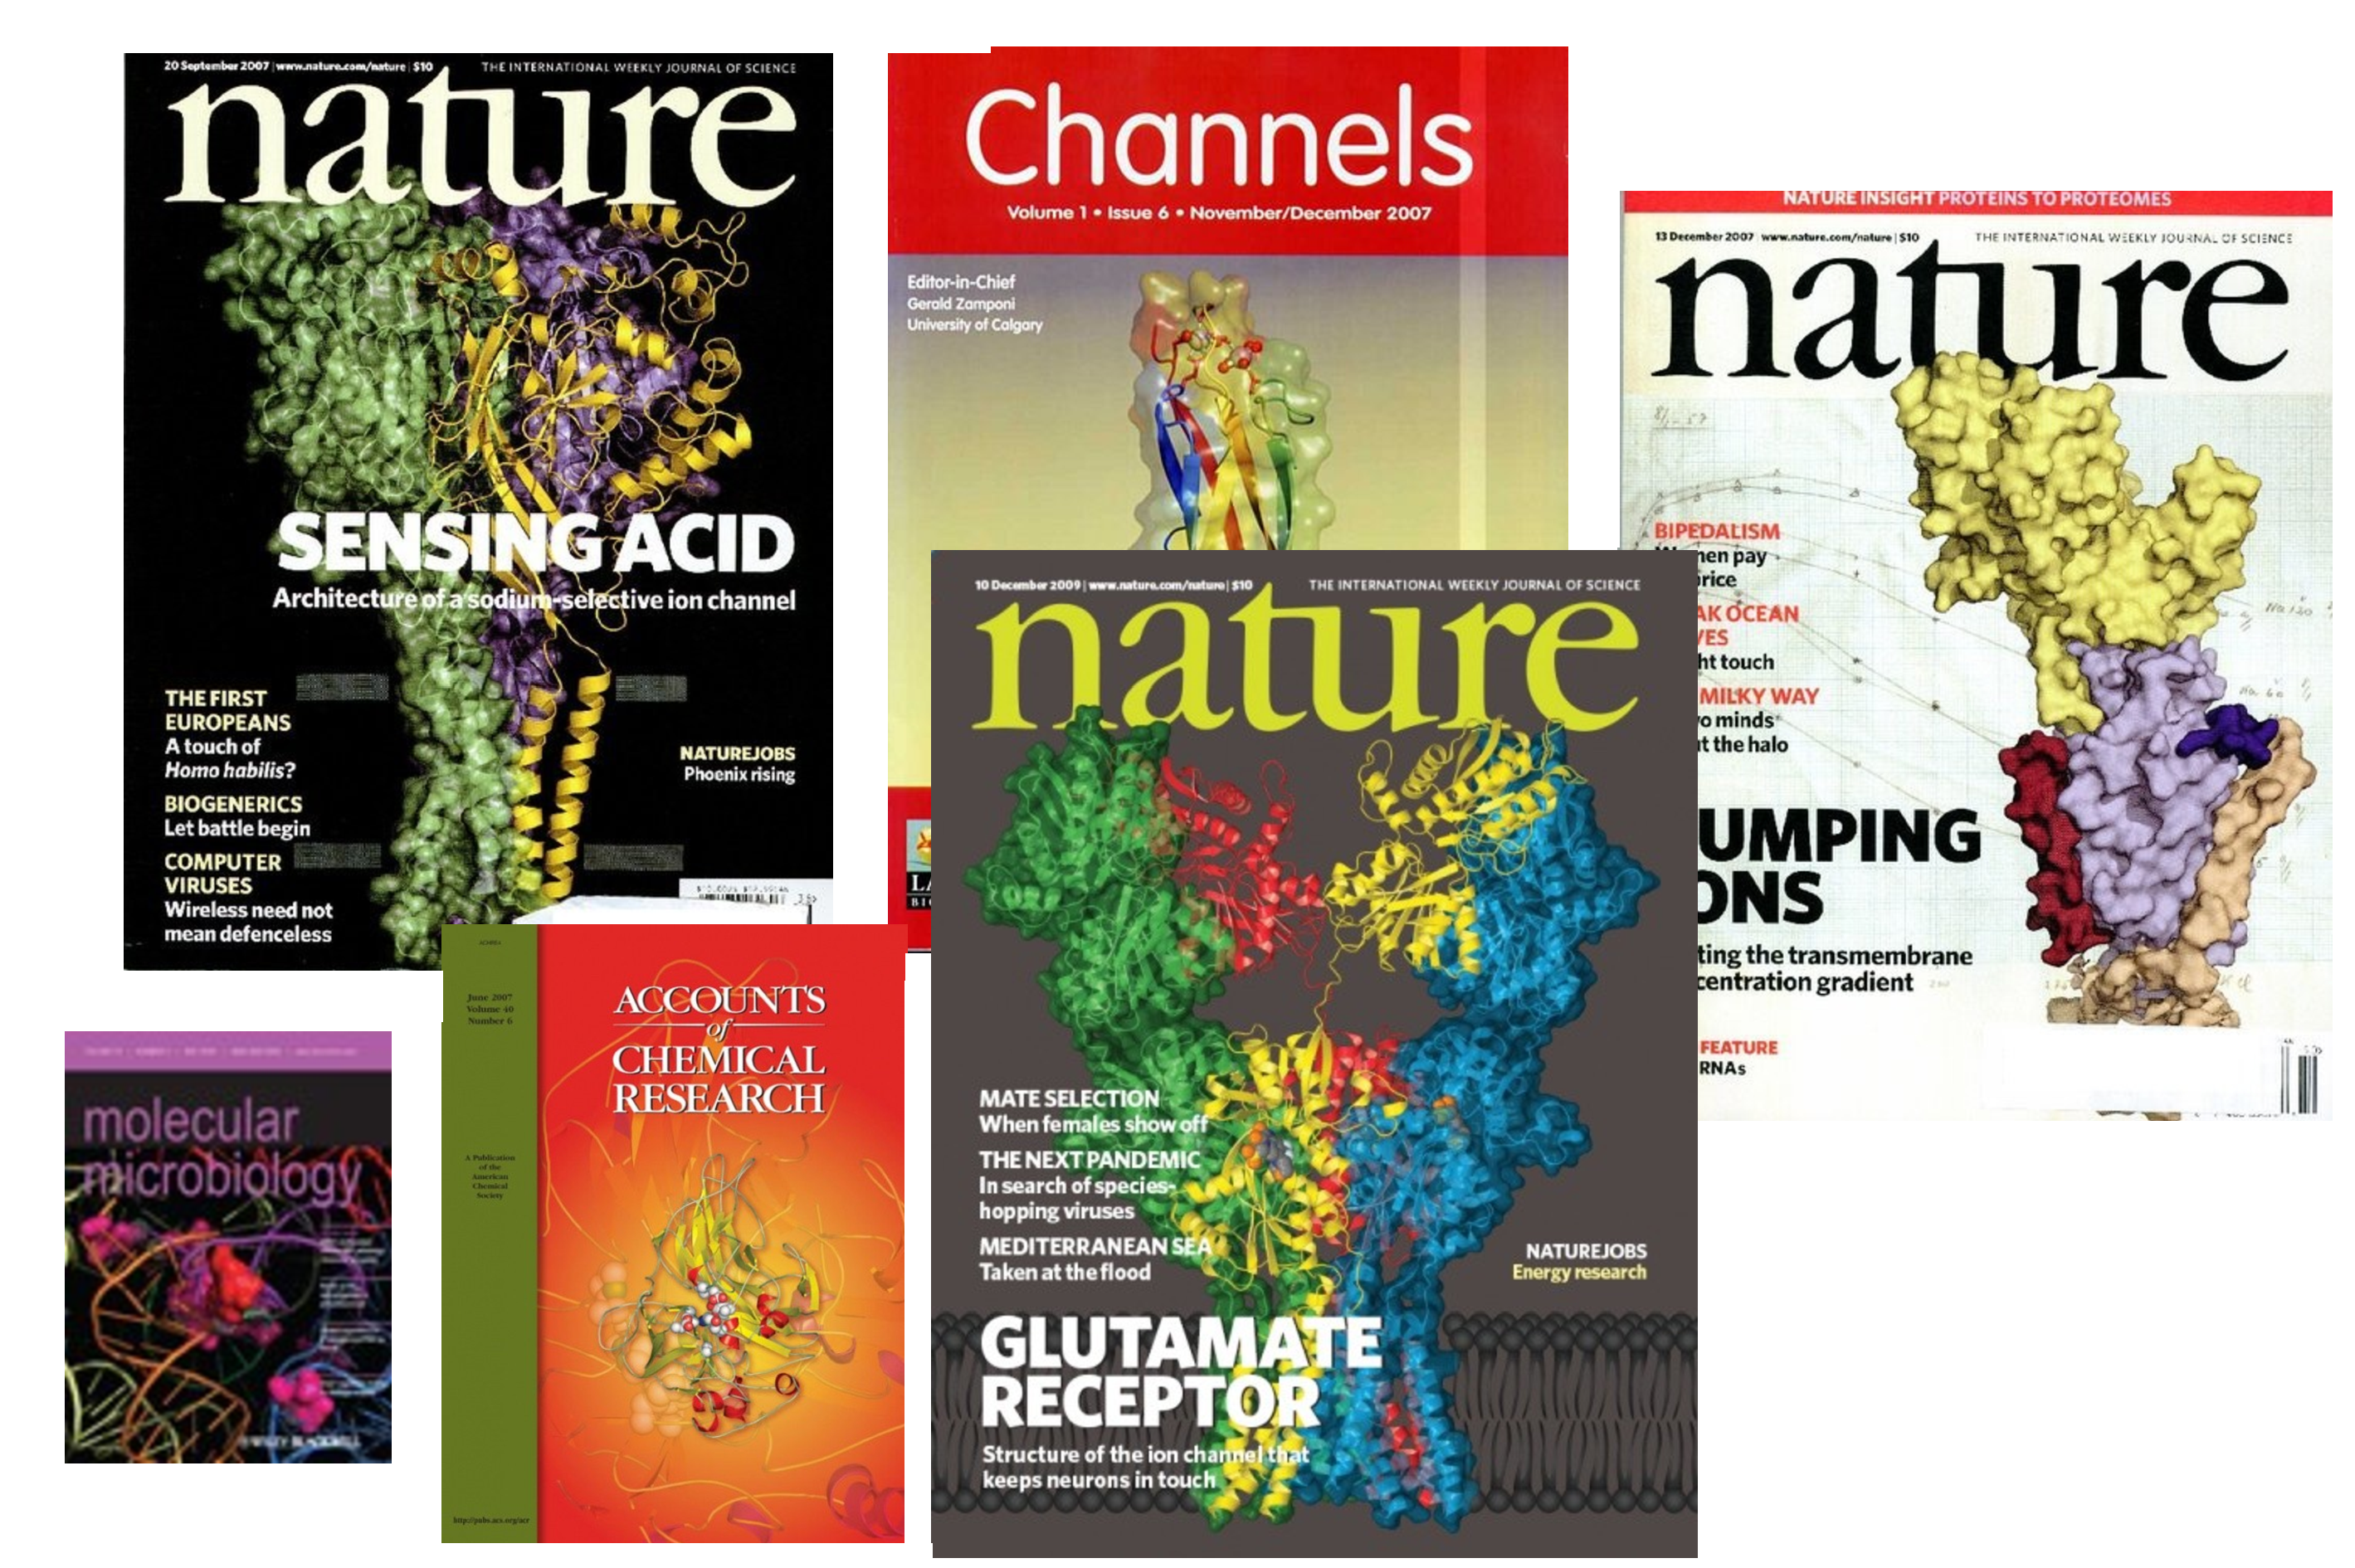
\includegraphics[height=0.75\textheight]{natures}
	  \end{center}
  \end{frame}

\begin{frame}{Для чего нужен PyMol}
	\begin{itemize}
	\item Визуализация pdb и прочих файлов с координатами атомов
	\item Изготовление высококачественных изображений
	\item Начальное редактирование структур
	\end{itemize}
\end{frame}

\begin{frame}{Системные требования}
	\textbf{Компьютер:} чем мощнее процессор и чем больше памяти, тем лучше\\
	\textbf{3D монитор} не обязателен, но поддерживается \\
	\textbf{Операционная система}: любая, под Linux проще установить, и он лучше работает с памятью.
\end{frame}

\begin{frame}{Как установить?}
	\begin{itemize}
		\item Компиляция из исходников:   http://pymol.svn.sourceforge.net/
		\item Установка бинарных пакетов в Ubuntu Linux: sudo apt-get install pymol
		\item Установка c Conda: conda install -c schrodinger pymol \\ 
		или  conda install -c conda-forge pymol-open-source
	   \end{itemize}
\end{frame}

\begin{frame}{PyMol - это GPL программа?}
	Да, PyMol это GPL-программа;
	\begin{itemize}
		\item исходный код доступен на sourceforge.net
		\item Бинарные пакеты для windows стоят денег и продаются: http://pymol.org/academic.html
		\item Бинарные пакеты для Linux собираются майтенерами
		\end{itemize}
	\end{frame}


  
  \section{Визуализация c PyMol}



  \begin{frame}{Меню объекта/выборки}
	\begin{center}
          \includegraphics[height=0.7\textheight]{pymol-ashl}
	  \end{center}
  \end{frame}


\section{Selections} 
\begin{frame}{Выборки}
	\begin{itemize}
		\item Можно задать с помощью кликов мыши, удерживая SHIFT
		\item Удобнее писать выражения в командной строке
		\end{itemize}

	Например:
	\textit{Select backbone, name ca+c+n }
\end{frame}

\begin{frame}{Операторы множеств}
	\begin{itemize}
		\item Логические операторы AND, OR,  NOT\\
					Операция OR может быть записана как ",". \\
				{ \tiny
					Упражнение: Документ PDB содержит описание структуры, состоящей из белка,
					фрагмента ДНК и молекул воды. Что получится, если задать следующие
				команды ?}\\
				\textit{
					select protein or dna \\
					select protein and dna\\
				select not water}
			\item Оператор WITHIN(...) \\
				\textit{
					select all within 3.5 of resi 20\\
				select s1, (byres n. ca) within 3.5 of resn LIG}
	\end{itemize}
\end{frame}

			 \begin{frame}[fragile]
				 \frametitle{Help selections}
{\tiny
	\hspace{0.5cm}	Длинное \hspace{2cm}Короткое
\begin{verbatim}
 name <atom names>           n. <atom names>
 resn <residue names>        r. <residue names>
 resi <residue identifiers>  i. <residue identifiers>
 chain <chain ID>            c. <chain identifiers>
 id <original-index>
 hydrogen                    h.
 all                         *
 visible                     v.
 hetatm
 byres <selection>           br. <selection>
 byobj <selection>           bo. <selection>
 around <distance>           a. <distance>
 expand <distance>           e. <distance>
 in <selection>
 like <selection>            l. <selection>

 <selection> within <distance> of <selection>
 <selection> w. <distance> of <selection> 
\end{verbatim}
}

Актуальное:\\
https://pymolwiki.org/index.php/Selection\_Algebra

\end{frame}

 \begin{frame}{Примеры выборок}
sel=select
    \begin{itemize}
   \item sel s1, n. ca and c. A : все атомы СА в цепи А
   \item sel s2, n. ca and (c. A or c. B) : атомы СА цепей А и В
   \item sel s3, resn GLU and resi 100 : остаток 100 если он GLU
   \item sel s4, resi 100-120+130 : атомы остатков 100-120 и 130
   \item sel s5, byres( name CG) : атомы остатков где есть CG
    \end{itemize}
\end{frame}

\begin{frame}{Иерархическое определение выборки}
		\begin{columns}
		\column{0.6\textwidth}
		Легко увидеть иерархию правым кликом по атому
		\column{0.4\textwidth}
		\includegraphics[height=0.3\textheight]{iearch.png}
		\end{columns}
		\textit{sel s1, a/102/cz}  : атом cz в остатке 102 \\
		\textit{sel s2, 100-120/N and c. A} : атомы N  в остатках 100-120 цепи а\\
		\textit{sel s3, a/100+120/} : все атомы остатков 100 и 120 в цепи А\\
\end{frame}

        
\begin{frame}{Трассировка лучей, команда ray }
	\small
	Подробно: \url{http://www.pymolwiki.org/index.php/Ray} \\
	\begin{columns}
		\column{0.3\textwidth}
		\includegraphics[height=0.3\textheight]{r1.png} \\
		No ray
		\column{0.3\textwidth}
		\includegraphics[height=0.3\textheight]{r2.png} \\
		ray\_trace\_mode,0
		\column{0.3\textwidth}
		\includegraphics[height=0.3\textheight]{r3.png} \\
		ray\_trace\_mode,1
	\end{columns} 
	\begin{columns}
		\column{0.3\textwidth}
		\includegraphics[height=0.3\textheight]{r4.png} \\
		ray\_trace\_mode,2
		\column{0.3\textwidth}
		\includegraphics[height=0.3\textheight]{r5.png} \\
		ray\_trace\_mode,3
	\end{columns}
\end{frame}

\begin{frame}[plain]
	\centering
	\includegraphicsfs{coord-zn}
\end{frame}

\begin{frame}{Настройки изображения}
	\url{http://www.pymolwiki.org/index.php/Category:Settings}
	\begin{itemize}
		\item PyMol содержит порядка 600 настроек
		\item Не все документированы
		\item Большинство интуитивно понятны
		\item Настройки доступны через меню или в командной строке набрать: \\
			\textit{set {первые буквы имени опции} и клавиша tab для достроения}
	\end{itemize}
\end{frame}

\begin{frame}{Примеры}
	\small
	\#initial setup\\
	\textcolor{blue!40!white}{viewport 600, 600} --- размер графического окна\\
	\textcolor{blue!40!white}{set auto\_zoom, off} --- не приближать новые объекты\\
	\textcolor{blue!40!white}{set auto\_show\_lines, off} --- не показывать линии автоматически\\
	\textcolor{blue!40!white}{set auto\_show\_selections, off} --- не показывать выборку автоматически\\
	\#cartoon parameters\\
	\textcolor{blue!40!white}{set cartoon\_fancy\_helices,1} --- изменение вида спиралей\\
	\textcolor{blue!40!white}{set cartoon\_highlight\_color, grey60} ---цвет внутренней стороны спиралей\\
	\textcolor{blue!40!white}{set cartoon\_dumbbell\_length,1.0} ---ширина ленты в спирали\\
	\textcolor{blue!40!white}{set cartoon\_rect\_length,1.40000} --- ширина ленты в бета\\
	\textcolor{blue!40!white}{set cartoon\_loop\_radius,0.3} --- толщина неструкт. участка\\ 
	\textcolor{blue!40!white}{set cartoon\_smooth\_loops=0} --- без сглаживания\\
\end{frame}

\begin{frame}[fragile]{\$HOME/.pymolrc}
\centering
\begin{lstlisting}
set sphere_scale,0.2
set async_builds, 1
set ribbon_width, 8
set antialias, 2
\end{lstlisting}
\end{frame}

\begin{frame}[fragile]{\$HOME/.pymolrc.py}
\centering
\begin{lstlisting}[language=Python]
from pymol import cmd
from pymol import stored

@cmd.extend
def superall(target):
    seleobjs = cmd.get_object_list('all')
    for o in seleobjs:
        if o != target:
            cmd.super(o,target)
            print(o)
\end{lstlisting}

\end{frame}

\section{Анимация}

\begin{frame}{Анимация в PyMol}
\small Если структура содержит более чем одну модель, то в PyMol можно
            анимировать движение молекулы переходом от одной модели к другой\\
\centering
 \inlineMovie[loop&autostart]{../../avi/nuc_mov_small.avi}{nuc_mov_small}{height=0.7\textheight}
\end{frame}


	\begin{frame}{Пример}
		\begin{itemize}
			\item Action->Preset->Technical (viewer gui)
			\item Scene->Store->F1
			\item zoom i. 90   \# увеличение остатка 90
			\item Scene->Store->F2
			\item Movie->Program->Scene Loop->Y-Rock->4 Seconds Each
			\item File-> Save movie
			\end{itemize}
		\end{frame}

		\begin{frame}{Результат}
          \begin{center} 
 \inlineMovie[loop&autostart]{../../avi/m2.mpg}{m2}{height=0.9\textheight}
          \end{center}
	  \end{frame}

	  \begin{frame}{Анимация, терминология}
		  \begin{itemize}
			  \item Объект и выборка : смотри выше
			  \item states: конформация или набор координат
			  \item scene: позиция камеры и отображение
			  \item frames: это кадры в анимации, содержит state и scene
			  \end{itemize}
			  \begin{center}
			  Movie panel: \hspace{.5cm}
          \includegraphics[width=0.2\textwidth]{an1.png}
	  \end{center}
	  \end{frame}

	  \begin{frame}{Анимация, команды}
		  \textcolor{blue!40!white}{mset 1 -55} : задать анимацию от 1 до 55 state на 55 кадров (frames) \\
		  \textcolor{blue!40!white}{mset 1 x90} : задать анимацию первого state от 1 до 90 кадров\\
		  \textcolor{blue!40!white}{mset 1 x30 1 -15 15 x30 15 -1 }: первые 30 кадров state 1, следующие 15 кадров это состояния 1-15, следующие 30 кадров состояние 15, следующие 15 кадров состояния от 15 до 1
	  \end{frame}

	  \begin{frame}{Анимация, команды}
			  mview : команда для создания ключевых точек \\
				  Пример :
		  \begin{itemize}
			  \item \textcolor{blue!40!white}{mset 1 x100}
			  \item \textcolor{blue!40!white}{frag leu}  \# создаём LEU
			  \item \textcolor{blue!40!white}{orient}    \# ориентируем его 
			  \item \textcolor{blue!40!white}{mview store} \# запоминаем ключевую точку
			  \item \textcolor{blue!40!white}{frame 100} \# переходим в кадр 100
			  \item \textcolor{blue!40!white}{zoom ID 10} \#  увеличиваем атом №10
			  \item \textcolor{blue!40!white}{mview store} \# запоминаем ключевую точку
			  \item \textcolor{blue!40!white}{mview reinterpolate} \# делаем интерполяцию
			  \end{itemize}
		  \end{frame}
		  
		  \begin{frame}{Результат mview}
          \begin{center} 
 \inlineMovie[loop&autostart]{../../avi/m4.mpg}{m4}{height=0.9\textheight}
          \end{center}
	  \end{frame}

	  \begin{frame}{Дополнительные команды}
		  \begin{itemize}
			  \item \textcolor{blue!40!white}{mmatrix} : устанавливает вид для первого кадра
			  \item \textcolor{blue!40!white}{util.mrock} : покачивание сцены на определённый угол 
			  \item \textcolor{blue!40!white}{util.mrock(start, finish, angle, phase, loop-flag) }
			  \item \textcolor{blue!40!white}{util.mroll} : вращение вокруг оси Y
			  \item \textcolor{blue!40!white}{util.mroll(start, finish, loop-flag)}
			  \item \textcolor{blue!40!white}{mdo} : (устарело) запуск какой-либо команды в заданном кадре
		   \end{itemize}
        Актульная информация:\\
        \textbf{https://pymolwiki.org/index.php/MovieSchool}

\end{frame}

	   \begin{frame}{Сохранение анимации}
		   \textbf{Старый путь: }\\
		   \textcolor{blue!40!white}{  set ray\_trace\_frames,1}\\
		   \textcolor{blue!40!white}{mpng mymovie}\\
		    Нужны программы avidemux, Virtual Dub, mencoder для того, чтобы собрать ролик с нужным сжатием (кодек)\\

			\textbf{Новый путь: File->Save movie }; есть недостаток, старый офис понимает только avi с определённым кодеком
		\end{frame}

		\section{Моделирование и редактирование в PyMol }

		\begin{frame}{Моделирование и редактирование в PyMol}
			\begin{itemize}
				\item Можно перемещать объекты и сохранять их новые координаты
				\item	Можно рассчитать вторичную структуру
				\item	Можно менять координаты отдельных атомов
				\item	Можно вносить мутации в белок (но не НК)
				\item	Можно конвертировать L->D аминокислоты
				\item	Можно добавлять протоны
				\item	Можно выравнивать в пространстве молекулы
				\item	Можно добавлять некоторые фрагменты из библиотеки и собственные
			\end{itemize}
		\end{frame}

		\begin{frame}{Перемещение объектов}
			Рекомендуемый порядок действий:\\
			\begin{itemize}
				\item \textcolor{blue!40!white}{set retain\_order} \# надо сохранить порядок атомов
				\item \textcolor{blue!40!white}{create newobj, sele} \# создаём новый объект, страховка
				\item \textcolor{blue!40!white}{translate [0,10,0], newobj} \# перемещаем
				\item \textcolor{blue!40!white}{rotate x,90,newobj} \# вращаем
				\item \textcolor{blue!40!white}{save newfile.pdb, newobj}
			\end{itemize}
			Операции по перемещению и вращению можно делать мышкой в режиме editing
		\end{frame}

		\begin{frame}{Изменение координат отдельных  атомов и объектов}

			\textcolor{blue!40!white}{alter\_state 1,(pdb1cse),x=x-10.0}\\
			Или 
			\textcolor{blue!40!white}{translate [0,10,0], A/100/NZ}

		\end{frame}

		\begin{frame}{Удаление связей,но не атомов}
			\begin{itemize}
				\item Выберите первый атом, ctrl+middle cliсk, выберите второй атом, ctrl+middle click

				\item И unbond или ctrl+D
			\end{itemize}

				\textbf{ Внимание! Координаты атомов не меняются, только исчезает изображение связи}
			
		\end{frame}

	\begin{frame}{Мутация аминокислот}
			\begin{itemize}
				\item Запустите wizard->mutagenesis 
				\item Выберите аминокислоту для мутации
				\item Справа выберите, на что мутировать
				\item Выберите ротамер с помощью управления movie
				\item Закончите процедуру с Apply
			\end{itemize}
	\end{frame}

     \begin{frame}{Добавление протонов}
			Работает с молекулами, т.е. объектами\\

			\textcolor{blue!40!white}{сreate gln, A/101/}\\
			\textcolor{blue!40!white}{h\_add gln}\\
			Или через меню action объекта.\\
			
			Есть вероятность, что протоны будут добавлены неверно, 
            если PyMol неправильно угадал валентность тяжёлых атомов.

	\end{frame}

	\begin{frame}{Суперпозиция в пространстве}
			Задача достаточно нетривиальная, и есть разные пути:\\

			Белки:\\
			 \textcolor{blue!40!white}{align, super, fit}\\
			Другое:\\
			 \textcolor{blue!40!white}{pair\_fit }\\
			Желательно указывать родственные атомы в молекулах\\
			 \textcolor{blue!40!white}{pair\_fit ( trna10 and resid 10:15 and name P ), ( ref4 and resid 10:15 and name P ) }
	 \end{frame}
		 
	\begin{frame}{Добавление органических фрагментов или а.к.}
			\begin{itemize}
				\item С помощью ctrl+middle click выделите шариком атом, к которому будет присоединяться фрагмент
				\item В меню Build выберите нужный фрагмент
				\item С помощью ctrl+left click выберите торсионный угол\\
					Или \\
				\item Создайте свою молекулу (ChemSketch)
				\item Сохраните как pkl в  <pymol\_path>/data/chempy/fragments
				\item \textcolor{blue!40!white}{editor.attach\_fragment('pk1','my\_fragment\_name',11,0)}\\
					  11 - это номер атома в фрагменте для связи
			\end{itemize}
	\end{frame}


	\begin{frame}{Sculpting, что ЭТО?}
			Это похоже на real-time оптимизатор геометрии, но это алгоритм, который старается сохранить значения длины связей, углов, торсионных углов при изменении координат. 
	\end{frame}

	\begin{frame}{Как запустить sculpting?}
			У вас достаточно мощный компьютер? Тогда:\\
			\begin{itemize}
				\item Переводим мышь в режим редактирования
				\item Выбираем "auto-sculpting" из меню Sculpting 
				\item Выбираем Sculpting из меню Wizard
				\item Выбираем центральный атом для модификаций Ctrl-middle-click 
				\item Тянем атом в любую сторону ctrl-left-click-and-drag 
			\end{itemize}
	\end{frame}

	\section{Скриптование в PyMol}

	\begin{frame}{Скриптование в PyMol}
			Возможны как скрипты из команд, так и скрипты на Python \\
			Запуск скриптов из команд:\\
			\textcolor{blue!40!white}{@ myfile.pml}\\
			Запуск скриптов на питоне:\\
			\textcolor{blue!40!white}{run myfile.py}
	\end{frame}

	\begin{frame}{Пример}
			\small
			\textcolor{blue!40!white}{
			fetch 1cll, async=0\\
			as lines, n. C+O+N+CA\\
			zoom i. 4+5\\
			mset 1 x1440\\
		    mview store\\
	        python}\\
			\textcolor{red}{for x in range(0,144):\\
				\hspace{0.5cm}  cmd.frame((10*x)+1)\\
			    \hspace{0.5cm}  cmd.zoom( "n. CA and i. " + str(x) + "+" + str(x+1))\\
			    \hspace{0.5cm}  cmd.mview("store")\\}
			\textcolor{blue!40!white}{
			python end\\
			frame 288\\
			mview store\\
		mview reinterpolate}\\
	\end{frame}

    \begin{frame}[plain]
        \includegraphicsfs{pymol-vscode}
    \end{frame}

    \fullFrameMovie[loop&autostart]{../../avi/r1111.mp4}{r1111}{\copyrightText{Какая-то муть}}


    
	  \begin{frame}{Объекты из Pymol можно использовать в разных 3D программах}
		  \begin{center}
			\includegraphics[height=0.5\textheight]{1lmp_2_small.png} 
			\includegraphics[height=0.5\textheight]{c_gold_small.png} 
			\includegraphics[height=0.5\textheight]{s_s_flame_black2_small.png}
		\end{center}
		\end{frame}

\begin{comment}
	  \begin{frame}{Или рисовать ручкой}
		  \begin{center}
			\includegraphics[width=1\textwidth]{sketchy-tamara} 
		\end{center}
		\end{frame}
\end{comment}

	  \begin{frame}[plain]
			\includegraphicsfs{sketchy-tamara} 
	  \end{frame}
\begin{comment}

\begin{frame}[plain]{}
    \begin{textblock*}{\paperwidth}(0\paperwidth,0\paperheight)
    \inlineMovie[loop&autostart]{../../avi/try4_vessel.avi}{surf}{width=1\textwidth}
    \end{textblock*}
\end{frame}
\end{comment}

    \fullFrameMovie[loop&autostart]{../../avi/try4_vessel.mp4}{try4_vessel}{\copyrightText{Анимация структуры в Blender}}
%	  \begin{frame}{Анимация структуры в Blender}
%          \begin{center} 
%    \movie[poster,autostart,width=0.72\linewidth, height=0.4\linewidth,loop]{%
%        \hspace{1cm}\includesvg{media-playback-start}
%           }{../avi/try4_vessel.avi}
%          \end{center}
%		\end{frame}
				  
%%%%%%%%%%%%%%%%%%%%%%%%%%%%%%%%%%%%%%%%
\begin{comment}

\end{comment}


%%===========================
	


